\chapter{Subsistema de transformación}

\section{Arquitectura del subsistema}

\begin{figure}[!htb]
	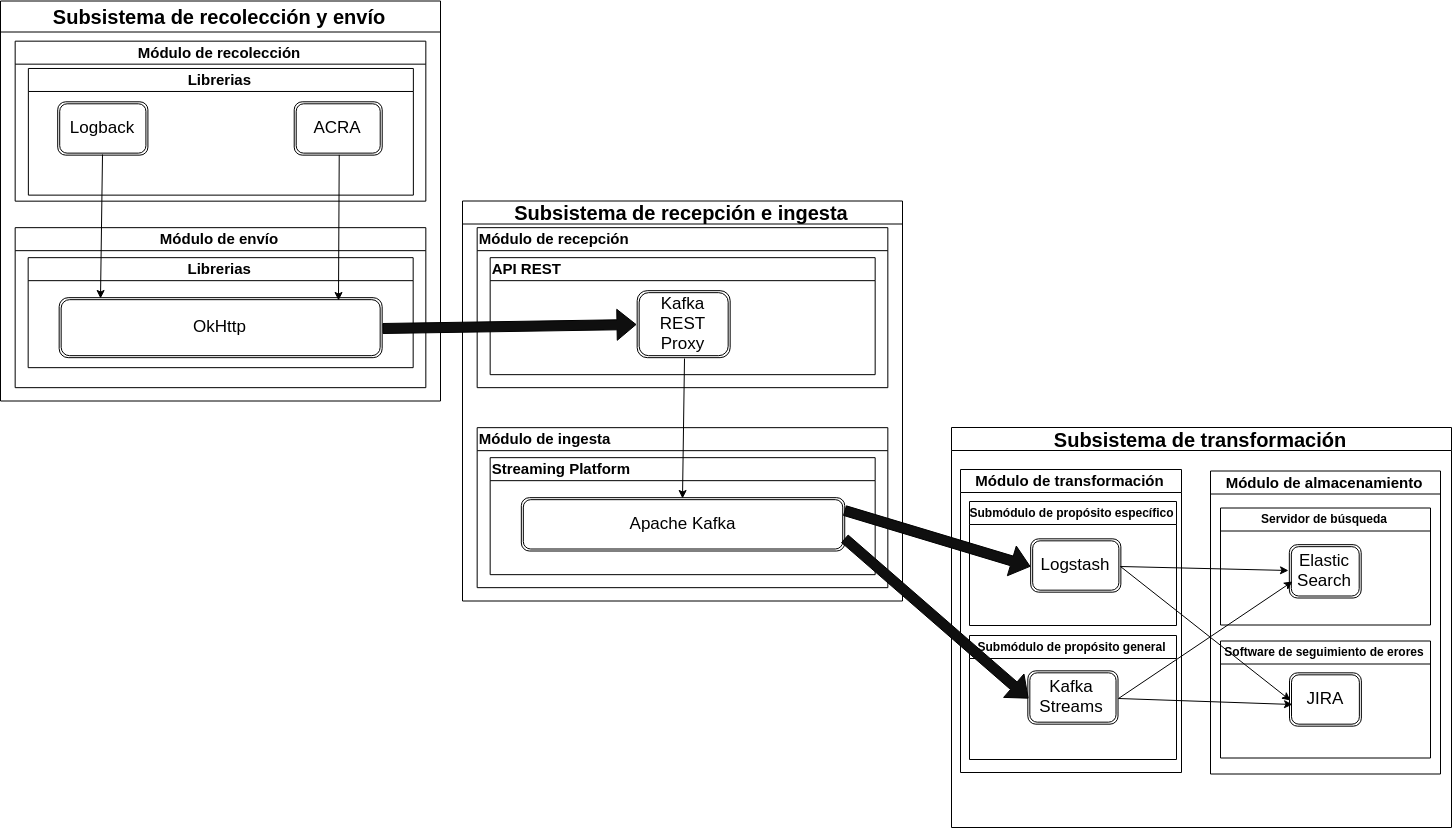
\includegraphics[width=\linewidth]{Moduloss-subtran.png}
	\caption{Vista general del sistema hasta el subsistema de transformación}
	\label{fig:subtra}
\end{figure}

El subsistema de transformación está formado por dos módulos, los cuales actúan fuera del dispositivo ubicuo. Esta es una división a nivel lógico y existe para reducir a problemas más simples el problema general, aunque nada impide que una herramienta implemente dos módulos. En la figura \ref{fig:subtra} se puede ver como se relacionan los módulos y las herramientas del subsistema. Las flechas indican el sentido del flujo de datos.

\subsection{Módulo de transformación}

El módulo de transformación es el encargado de consumir los datos del módulo de ingesta, hacer las transformaciones deseadas a los datos y publicarlas en el módulo de almacenamiento. Este módulo no almacena de forma persistente los datos.

Este módulo es necesario ya que nos ayuda a crear información de valor con los eventos extraídos, a parte de generar la información en un formato que el módulo de almacenamiento acepte.

\subsection{Módulo de almacenamiento}

El módulo de almacenamiento es el encargado de recibir los datos transformados del módulo de transformación y almacenarlos para que puedan ser consumidos por otros sistemas o aplicaciones.

Este módulo es necesario ya que es el encargado de almacenar de forma persistente los datos transformados y sin él otros sistemas no podrían consumir los datos transformados.


\section{Estructura del subsistema}

La estructura de este subsistema puede variar mucho dependiendo de los datos que se quieran procesar, en nuestro casos son logs y crashlogs, por lo que la estructura utilizada ha de ser capaz de transformar de forma eficaz logs y crashlogs, pero la elección de la estructura no ha de condicionar el propósito del sistema. Aunque el sistema del proyecto ha de trabajar con eventos, se ha buscado la solución más general para tener lo más cercano a un sistema de propósito general, de esta manera se podrán procesar otro tipo de datos cuando sea necesario. Se ha de tener en cuenta que la elección del módulo de almacenamiento no se ha tomado en este proyecto, sino que este sistema se ha tenido que acoplar con un módulo de almacenamiento existente en la empresa, por lo que la elección estructural del módulo de transformación se ha visto en parte condicionada por el módulo de almacenamiento existente.


\subsection{Módulo de transformación}

Para el módulo de transformación se ha buscado por un lado, que sea eficaz transformando logs y crashlogs y por otro que sea lo más general posible para soportar en el futuro la transformación de otro tipo de datos, por lo que la solución encontrada pasa por aprovechar la existencia de un módulo de ingesta extremadamente versátil y dividir en submódulos, que pueden colaborar entre ellos, el módulo de transformación. Así pues, los elementos a nivel estructural han de encajar en esta división.
\\\\
Como se puede apreciar en la Figura \ref{fig:subtra}, el módulo de transformación se divide en dos submódulos:

\subsubsection{Submódulo de propósito general}
El submódulo de propósito general es capaz de transformar todo tipo de datos, ya sean eventos u otra cosa. Este submódulo se ha añadido para dotar al sistema de generalidad transformando datos. Este submódulo es capaz de hacer transformaciones stateful como agregaciones, joins y windowing, o transformaciones stateless como filtering y mapping, todas ellas en tiempo real. A parte, este submódulo es fácilmente escalable, desplegable e integrable con el submódulo de ingesta. La solución escogida ha sido, en vez de una estructura pasiva a la que se le envían lotes de trabajo para que los procese, un solución activa en la que una aplicación con el uso de alguna librería sea capaz de consumir los datos del módulo de ingesta, transformarlos, y publicarlos en el módulo de almacenamiento. Por lo que a nivel estructural este submódulo es una aplicación que utiliza una librería de stream processing.

\subsubsection{Submódulo de propósito específico}
El submódulo de propósito específico es capaz de transformar un tipo de datos en concreto, en el caso de este proyecto eventos. Este módulo hace transformaciones que requieren una potencia de cálculo menor que las transformaciones que puede hacer el submódulo de propósito general. Las transformación que principalmente efectúa es un enriquecimiento para que los datos sean aceptados en el módulo de destino o para que el submódulo de propósito general haga transformaciones más potentes con los datos ya enriquecidos. \\\\


Estos dos submódulos pueden cooperar entre ellos. Por ejemplo, los datos podrían pasar primero por el submódulo de propósito general aplicarles la transformación pertinente y luego pasarlos al submódulo de propósito específico enriquecerlos y pasarlos al módulo de almacenamiento.
\\
Esta división en submódulos hace que la aplicación sea viable para todos los casos de uso, ya sea un caso de uso que requiera poca potencia de procesado o mucha potencia de procesado. Con esta división se ajustan bastante los costes a la complejidad del procesado, si el procesado es simple, el precio será bajo, si el procesado es complejo el precio será alto, por lo que no existe un umbral a partir del cual salga a cuenta hacer el procesado de los datos, siempre lo es. Es más, no es necesario utilizar los dos submódulos, quizás con las transformaciones que ofrece uno de los dos módulos es suficiente. 
\\
Para que la división en submódulos sea tan versátil es importante que el submódulo de propósito general se pueda adaptar a la complejidad del problema, es decir, que para problemas simples no utilice una cantidad elevada de recursos que hagan que ese procesado no salga a cuenta. No se habla del submódulo de propósito específico ya que este submódulo depende en gran medida del módulo de almacenamiento, por lo que habrán situaciones en las que este submódulo tenga que estar sobredimensionado por culpa del módulo de almacenamiento, pero se pueden compensar los costes gracias al submódulo de propósito general.

%% !!!si tienes uno de caracter especifico pasivo uno de caracter general activo, el de caracter general es escalable y adaptable. Tienes un módulo específico potente y uno general ligeramente menos potente que la media pero mucho más barato, por lo que los dos submódulos se complementan para dar un sistema escalable y versatil.


\subsection{Módulo de almacenamiento}
El módulo de almacenamiento nos venía dado por la empresa. La empresa ya utilizaba un módulo de almacenamiento en concreto y el sistema se ha de integrar con él. El módulo de almacenamiento lo integra una aplicación de seguimiento de errores y un servidor de búsqueda. Los dos elementos tienen bases de datos, pero para acceder a ellas se ha de hacer a través de los puntos de entrada que disponen, API REST en este caso. El sistema se ha de integrar con este módulo.
\section{Herramientas utilizadas}

\subsection{Módulo de transformación}
\subsubsection{Submódulo de propósito general}
Para el submódulo de propósito general se ha decidido utilizar Kafka Streams\cite{Tfg:kafkastreams} ya que a parte de cumplir las necesidades estructurales, por las siguientes razones:

\begin{itemize}
	\item \textbf{Proporciona una abstracción de alto nivel para hacer las transformaciones}. Repercute en el tiempo necesario para programar la solución deseada.
	
	\item \textbf{Hace un Stream Processing real, no hace micro-batching}. Por lo que las latencias de procesado pueden ser muy bajas.
	
	\item \textbf{Se integra sin problemas con Kafka}. No se produce un cuello de botella entre las dos herramientas.
	
	\item \textbf{Es una librería de Java}. Una aplicación en Java que utiliza Kafka Streams es la que hace la transformación de los datos, por lo que la aplicación se podrá desplegar en máquinas que soporten Java, no es necesario desplegar un cluster para realizar las transformaciones, aunque nada impide desplegar uno. Es altamente escalable puesto que si se necesita más potencia de cálculo tan solo se ha de desplegar otra instancia de la aplicación en otra máquina o en una en la que ya está corriendo la aplicación.
\end{itemize}



\subsubsection{Submódulo de propósito específico}
Para el submódulo de propósito general se ha decidido utilizar Logstash puesto que se integra perfectamente con Kafka y Elastic Search, y hace una transformación específica para eventos, ofreciendo transformaciones bastante útiles para el caso de los eventos.

\subsection{Módulo de almacenamiento}
Las herramientas que componen el módulo de almacenamiento son Elastic Search, en el cual se almacenan logs y crashlogs, y JIRA, en el cual se alamacenan tan solo crashlogs. Estas herramientas ya estaban presentes en la empresa.

\section{Configuración del subsistema}

\subsection{Módulo de transformación}
La configuración de este módulo depende de la transformación que se quiera hacer a los datos. Para comprobar el funcionamiento del módulo y simplificar el problema, se hacen transformaciones simples que puedan ser demostrables el día de la demostración.
\\\\
Para los logs, lo que se pretende es que se enriquezcan. En concreto, los logs entran como un objeto JSON, y las claves de este objeto son tan solo un carácter, lo que se quiere es reemplazar las claves por una palabra que identifique mejor que es cada parte del objeto JSON y luego publicarlo en Elastic Search. Para este caso haciendo uso del submódulo de propósito específico nos basta. Se ha configurado Logstash para que sea capaz de consumir los datos del topic \textit{logs} de Kafka, transformarlos y publicarlos en Elastic Search. 
\\\\
Para los crashlogs, lo que se pretende es que cuando se produzca el mismo crashlog X veces durante un periodo de tiempo de Y segundos, se genere un ticket en JIRA que contenga los datos más relevantes de este crashlog. A parte, también se quiere que todos los crashlogs que se produzcan, se publiquen en Elastic Search. Para este caso se hace uso de los dos submódulos. El submódulo de propósito general se encarga de controlar si se produce el mismo crashlog X veces durante un periodo de tiempo de Y segundos, y de generar el ticket en JIRA. El submódulo de propósito específico se encarga de publicar todos los crashlogs en Elastic Search.

\subsection{Módulo de almacenamiento}
Este módulo ya está configurado por la empresa, por lo que la configuración que se va a hacer es una que permita ver que el sistema funciona como se espera el día de la presentación.
\\\\
En JIRA se ha creado un proyecto, en el cual se publican los tickets con la información sobre los crashlogs.
En Elastic Search se han creado dos índices, uno para los logs y otro para los crashlogs.

\section{Integración con el entorno}
El módulo de transformación se ha de integrar con un módulo de almacenamiento ya existente en la empresa, en concreto se ha de integrar con JIRA y con Elastic Search. De la integración con JIRA se espera que el sistema sea capaz de crear un ticket en JIRA con información obtenida de los eventos. De la integración con Elastic Search se espera que el sistema sea capaz de publicar información, obtenida de las alertas, en dos índices de Elastic Search con el objetivo de que la información publicada sea visible en Kibana.





